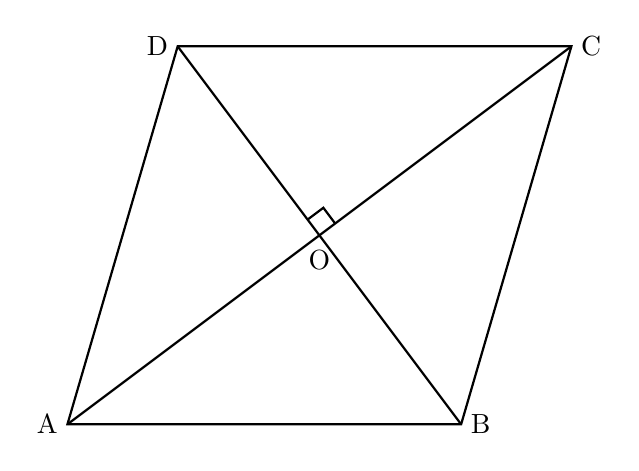
\begin{tikzpicture}[scale=1]

    % Define the vertices of the parallelogram
    % The coordinates are mathematically derived to ensure the diagonals intersect at exactly 90 degrees as shown.
    \coordinate (A) at (0,0);
    \coordinate (B) at (5,0);
    \coordinate (C) at (6.4,4.8);
    \coordinate (D) at (1.4,4.8);

    % Define the intersection point of the diagonals
    \coordinate (O) at (3.2,2.4);

    % Draw the outer boundary of the parallelogram
    \draw[thick] (A) -- (B) -- (C) -- (D) -- cycle;

    % Draw the diagonal segments
    \draw[thick] (A) -- (C);
    \draw[thick] (B) -- (D);

    % Draw the right-angle symbol at the intersection O (specifically inside angle DOC)
    % Exact coordinates for a square symbol of size 0.25 aligned with the diagonals
    \draw[thick] (3.05, 2.60) -- (3.25, 2.75) -- (3.40, 2.55);

    % Place the labels exactly where they appear in the image
    \node[left] at (A) {A};
    \node[right] at (B) {B};
    \node[right] at (C) {C};
    \node[left] at (D) {D};
    
    % Label O is placed just below the intersection
    \node[below, yshift=-2pt] at (O) {O};

\end{tikzpicture}